% GNUPLOT: LaTeX picture with Postscript
\begingroup
  \makeatletter
  \providecommand\color[2][]{%
    \GenericError{(gnuplot) \space\space\space\@spaces}{%
      Package color not loaded in conjunction with
      terminal option `colourtext'%
    }{See the gnuplot documentation for explanation.%
    }{Either use 'blacktext' in gnuplot or load the package
      color.sty in LaTeX.}%
    \renewcommand\color[2][]{}%
  }%
  \providecommand\includegraphics[2][]{%
    \GenericError{(gnuplot) \space\space\space\@spaces}{%
      Package graphicx or graphics not loaded%
    }{See the gnuplot documentation for explanation.%
    }{The gnuplot epslatex terminal needs graphicx.sty or graphics.sty.}%
    \renewcommand\includegraphics[2][]{}%
  }%
  \providecommand\rotatebox[2]{#2}%
  \@ifundefined{ifGPcolor}{%
    \newif\ifGPcolor
    \GPcolorfalse
  }{}%
  \@ifundefined{ifGPblacktext}{%
    \newif\ifGPblacktext
    \GPblacktexttrue
  }{}%
  % define a \g@addto@macro without @ in the name:
  \let\gplgaddtomacro\g@addto@macro
  % define empty templates for all commands taking text:
  \gdef\gplbacktext{}%
  \gdef\gplfronttext{}%
  \makeatother
  \ifGPblacktext
    % no textcolor at all
    \def\colorrgb#1{}%
    \def\colorgray#1{}%
  \else
    % gray or color?
    \ifGPcolor
      \def\colorrgb#1{\color[rgb]{#1}}%
      \def\colorgray#1{\color[gray]{#1}}%
      \expandafter\def\csname LTw\endcsname{\color{white}}%
      \expandafter\def\csname LTb\endcsname{\color{black}}%
      \expandafter\def\csname LTa\endcsname{\color{black}}%
      \expandafter\def\csname LT0\endcsname{\color[rgb]{1,0,0}}%
      \expandafter\def\csname LT1\endcsname{\color[rgb]{0,1,0}}%
      \expandafter\def\csname LT2\endcsname{\color[rgb]{0,0,1}}%
      \expandafter\def\csname LT3\endcsname{\color[rgb]{1,0,1}}%
      \expandafter\def\csname LT4\endcsname{\color[rgb]{0,1,1}}%
      \expandafter\def\csname LT5\endcsname{\color[rgb]{1,1,0}}%
      \expandafter\def\csname LT6\endcsname{\color[rgb]{0,0,0}}%
      \expandafter\def\csname LT7\endcsname{\color[rgb]{1,0.3,0}}%
      \expandafter\def\csname LT8\endcsname{\color[rgb]{0.5,0.5,0.5}}%
    \else
      % gray
      \def\colorrgb#1{\color{black}}%
      \def\colorgray#1{\color[gray]{#1}}%
      \expandafter\def\csname LTw\endcsname{\color{white}}%
      \expandafter\def\csname LTb\endcsname{\color{black}}%
      \expandafter\def\csname LTa\endcsname{\color{black}}%
      \expandafter\def\csname LT0\endcsname{\color{black}}%
      \expandafter\def\csname LT1\endcsname{\color{black}}%
      \expandafter\def\csname LT2\endcsname{\color{black}}%
      \expandafter\def\csname LT3\endcsname{\color{black}}%
      \expandafter\def\csname LT4\endcsname{\color{black}}%
      \expandafter\def\csname LT5\endcsname{\color{black}}%
      \expandafter\def\csname LT6\endcsname{\color{black}}%
      \expandafter\def\csname LT7\endcsname{\color{black}}%
      \expandafter\def\csname LT8\endcsname{\color{black}}%
    \fi
  \fi
  \setlength{\unitlength}{0.0500bp}%
  \begin{picture}(8640.00,6480.00)%
    \gplgaddtomacro\gplbacktext{%
      \csname LTb\endcsname%
      \put(2779,1418){\makebox(0,0)[r]{\strut{}\bfseries F=1/2}}%
      \put(2779,2204){\makebox(0,0)[r]{\strut{}\bfseries F=3/2}}%
      \put(2911,484){\makebox(0,0){\strut{} 0}}%
      \put(3830,484){\makebox(0,0){\strut{} 50}}%
      \put(4749,484){\makebox(0,0){\strut{} 100}}%
      \put(5667,484){\makebox(0,0){\strut{} 150}}%
      \put(6586,484){\makebox(0,0){\strut{} 200}}%
      \put(2405,3459){\rotatebox{-270}{\makebox(0,0){\strut{}Zeeman shift (MHz)}}}%
      \put(4748,154){\makebox(0,0){\strut{}magnetic field (G)}}%
      \put(1441,1902){\makebox(0,0)[l]{\strut{}$\mathbf{2S_{1/2}}$}}%
      \put(2176,4777){\makebox(0,0)[l]{\strut{}$\mathbf{2P_{3/2}}$}}%
      \put(6770,896){\makebox(0,0)[l]{\strut{}$| 1 \rangle \equiv | 1/2,\hspace{3mm}  1/2;              -1/2, \hspace{3mm} 1 \rangle$}}%
      \put(6770,1135){\makebox(0,0)[l]{\strut{}$| 2 \rangle \equiv | 1/2,              -1/2;              -1/2, \hspace{3mm} 0 \rangle$}}%
      \put(6770,1399){\makebox(0,0)[l]{\strut{}$| 3 \rangle \equiv | 3/2,              -3/2;              -1/2,              -1 \rangle$}}%
      \put(6770,2381){\makebox(0,0)[l]{\strut{}$| 4 \rangle \equiv | 3/2,              -1/2; \hspace{3mm} 1/2,              -1 \rangle$}}%
      \put(6770,2621){\makebox(0,0)[l]{\strut{}$| 5 \rangle \equiv | 3/2,\hspace{3mm}  1/2; \hspace{3mm} 1/2, \hspace{3mm} 0 \rangle$}}%
      \put(6770,2860){\makebox(0,0)[l]{\strut{}$| 6 \rangle \equiv | 3/2,\hspace{3mm}  3/2; \hspace{3mm} 1/2, \hspace{3mm} 1 \rangle$}}%
      \put(7505,1902){\makebox(0,0)[l]{\strut{}$| F, m_{F}; m_{S}, m_{I} \rangle$}}%
      \put(9894,2621){\makebox(0,0)[l]{\strut{}$m_{J}= +1/2 $}}%
      \put(9894,1183){\makebox(0,0)[l]{\strut{}$m_{J}= -1/2 $}}%
      \put(6770,3460){\makebox(0,0)[l]{\strut{}$| m_{J}=              -3/2 ;\ m_{I}=-1,0,1 \rangle$}}%
      \put(6770,4346){\makebox(0,0)[l]{\strut{}$| m_{J}=              -1/2 ;\ m_{I}=-1,0,1 \rangle$}}%
      \put(6770,5233){\makebox(0,0)[l]{\strut{}$| m_{J}=\hspace{3mm}  1/2 ;\ m_{I}=-1,0,1 \rangle$}}%
      \put(6770,6119){\makebox(0,0)[l]{\strut{}$| m_{J}=\hspace{3mm} +3/2 ;\ m_{I}=-1,0,1 \rangle$}}%
      \put(4565,4035){\rotatebox{-20}{\makebox(0,0)[l]{\strut{}\textcolor{red}{\small -2.8 MHz/G}}}}%
      \put(4932,1159){\rotatebox{-10}{\makebox(0,0)[l]{\strut{}\textcolor{red}{\small -1.4 MHz/G}}}}%
    }%
    \gplgaddtomacro\gplfronttext{%
    }%
    \gplbacktext
    \put(0,0){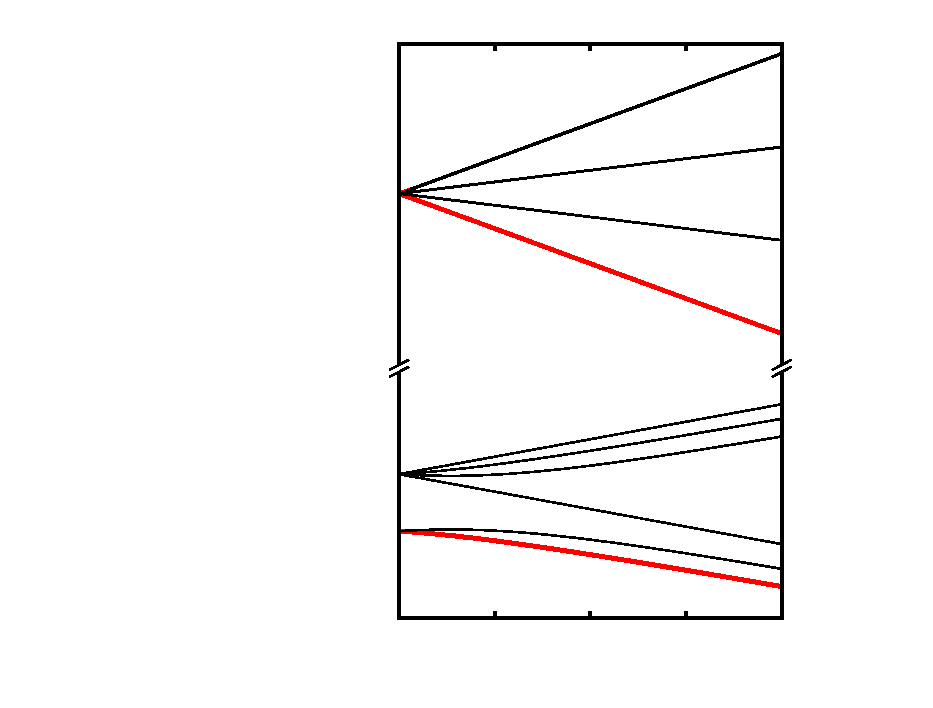
\includegraphics{01}}%
    \gplfronttext
  \end{picture}%
\endgroup
